\chapter{Интеграционное тестирование}

В данной части работы будет осуществлено тестирование модулей сервера, обрабатывающие запросы, взаимодействующие с базой данных, в данных тестах рассмотрены сценарии, в которых совместно используются несколько модулей.

\section{Тестирование модулей}
В тестах ниже используются методы основных классов упомянутых выше. 


Интеграционные тесты описаны в таблице \ref{tab:maintable}.

\begin{table} 
\caption{\label{tab:maintable}Интеграционное тестирование}
\begin{center}
\begin{tabular}{|l|p{10cm}|}
\hline
\multicolumn{2}{|c|}{Удаление существующей подписки} \\
\hline
Запрос & \{userid: 777, groupname: MyGroup, groupid: 111\} \\
Ожидаемый результат & Удаление исполнителя из подписки  \\
Используемые классы & UserActions,SubscriptionActions,GroupActions \\
\hline
\multicolumn{2}{|c|}{Удаление несуществующей подписки} \\
\hline
Запрос & \{userid:777, groupdid:111, wrongid:1111, groupname: NoGroup \} \\
Ожидаемый результат & Список подписок остается тем же, функция удаления возвращает результат = null  \\
Используемые классы & UserActions,SubscriptionActions,GroupActions \\
\hline
\multicolumn{2}{|c|}{Вывод подписок пользователя} \\
\hline
Запрос & \{userid: 999, groupid:222, groupname: RandGroup \} \\
Ожидаемый результат & Вывод подписок пользователя с userid=999 \\
Используемые классы & UserActions,SubscriptionActions  \\
\hline
\multicolumn{2}{|c|}{Удаление всех подписок одного пользователя} \\
\hline
Запрос & \{userid: 777, groupname: MyGroup, groupid:111 \} \\
Ожидаемый результат & даление подписок пользователя с id=777 \\
Используемые классы & UserActions,SubscriptionActions,GroupActions  \\
\hline
\multicolumn{2}{|c|}{Удаление всех подписок одного пользователя, не затрагивая чужие} \\
\hline
Запрос & \{userid: 777, additional userid: 787, groupname: MyGroup, groupid:111 \} \\
Ожидаемый результат &Удаление подписок пользователя с id=777, подписки пользователя с id=787 остались прежними \\
Используемые классы & UserActions,SubscriptionActions,GroupActions  \\
\hline
\multicolumn{2}{|c|}{Добавление концерта новой группы} \\
\hline
Запрос & \{userid: 777, groupname: RandGroup, groupid:888, Concert: EmptyConcert\} \\
Ожидаемый результат & Добавление группы в таблицу групп и добавление концерта этой группы в таблицу концертов \\
Используемые классы & UserActions,SubscriptionActions,GroupActions, ConcertActions  \\
\hline
\multicolumn{2}{|c|}{Добавление концерта существующей группы} \\
\hline
Запрос & \{userid: 777, groupid:888, Concert: EmptyConcert\} \\
Ожидаемый результат & Добавление концерта группы в таблицу концертов \\
Используемые классы & UserActions,SubscriptionActions,GroupActions, ConcertActions  \\
\hline

\end{tabular}
\end{center}
\end{table} 
\newpage
\section{Покрытие}
\begin{figure}
	\centering
	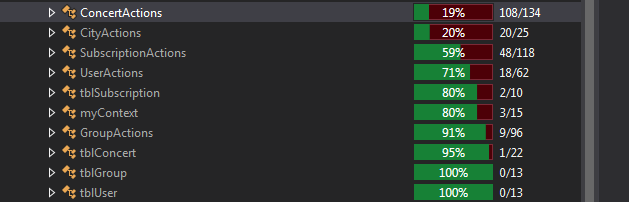
\includegraphics[scale=1]{CoverIntegration.PNG}
	\caption{Покрытие после модульных тестов и интеграционных}
	\label{image:cover-integration}
\end{figure}